%\vspace{-0.05in}
\section{BW-AWARE Page Placement}
\label{bwawareplacement}
%\vspace{-0.05in}
Using all available memory bandwidth is a key driver to maximizing 
performance for many GPU workloads.
To exploit this observation, we propose a new OS page placement algorithm which
accounts for the bandwidth differential between different bandwidth-optimized and 
capacity-optimized memories
when making page placement decisions.  This section discusses the need,
implementation, and results for a bandwidth-aware (BW-AWARE) page placement
policy for systems where the application footprint fits within BO memory, the
common case for GPU workloads today.  Later in Section~\ref{binaryinstrument},
we discuss an extension to BW-AWARE placement for systems where memory placement
decisions are constrained by the capacity of the
bandwidth-optimized memory.  Both HPC systems trying to maximize in-memory
problem footprint and mobile systems which are capacity limited by cost and
physical part dimensions may soon encounter these capacity constraints with
heterogeneous memories.

\subsection{Bandwidth Maximized Page Placement}
\label{unconstrained}
%\vspace{-0.05in}
The goal of bandwidth-aware page placement is to enable a GPU
to effectively use the total combined bandwidth of {\color{black}\emph{all} the} memory in the
system.  Because GPUs are able to hide high memory latency without stalling
their pipelines, all memories in a system can be used to service GPU requests, 
even when those memories are off-package or require one or more hops
through a system interconnect to access.
To exploit bandwidth-heterogeneous memories,
our BW-AWARE policy places physical memory pages in the ratio of aggregate 
bandwidths of the memories in the system without requiring any knowledge of page
access frequency. Below we derive that this placement policy is optimal for maximizing
bandwidth.

Consider a system with bandwidth-optimized and capacity-optimized
memories with bandwidths $b_B$ and $b_C$ respectively, where unrestricted
capacity of both memories are available. Let $f_B$ represent fraction of data
placed in the BO memory and $1-f_B$ in the CO memory.  Let us assume there are total of
N memory accesses uniformly spread among different pages. Then the total amount
of time spent by the BO memory to serve $N*f_B$ memory accesses is $N*f_B/b_B$ and
that by the CO memory to serve $N(1-f_B)$ memory accesses is $N(1-f_B)/b_C$.  Since
requests to these two memories are serviced in parallel, the total time T to serve the
memory requests is: 
%\[
%T=max(N*f_B/b_B, N(1-f_B)/b_C)
%\]
$$T=max(N*f_B/b_B, N(1-f_B)/b_C)$$
To maximize performance, T must be minimized. Since, $N*f_B/b_B$ and
$N(1-f_B)/b_C$ are linear in $f_b$ and $N*f_B/b_B$ is increasing function while
$N(1-f_B)/b_C$ is decreasing, the minimum of T occurs when both are equal:
%\[T_{opt}=N*f_B/b_B = N(1-f_B)/b_C\]
$$T_{opt}=N*f_B/b_B = N(1-f_B)/b_C$$
Therefore,
%\[f_{Bopt}=b_B/(b_B+b_C)\]
$$f_{Bopt}=b_B/(b_B+b_C)$$

Because we have assumed that all pages are accessed uniformly, the optimal page
placement ratio is the same as the bandwidth service ratio between the bandwidth-optimized
and capacity-optimized memory pools. From this derivation we make two additional
observations.  First, BW-AWARE placement will generalize to an optimal policy
where there are more than two technologies by placing pages in the bandwidth ratio
of all memory pools. Second, a practical implementation
of a BW-AWARE policy must be aware of the bandwidth provided by the various
memory pools available within a system. Hence there is a need for a new System
Bandwidth Information Table (SBIT), much like there is already a ACPI System
Locality 
Information Table (SLIT) which exposes memory latency information to the operating
system today. We will re-visit the assumption of uniform page access later in Section~\ref{annotation}.  

\begin{table}[t]
\begin{center}
\begin{small}
\begin{tabular}{|l|l|}
\hline
Simulator & GPGPU-Sim 3.x\\
\hline
GPU Arch & NVIDIA GTX-480 Fermi-like\\
\hline
GPU Cores& 15 {\color{black}SMs} @ 1.4Ghz\\
\hline
L1 Caches & 16kB/SM \\
\hline
L2 Caches & Memory Side 128kB/DRAM Channel\\
\hline
L2 MSHRs & 128 Entries/L2 Slice\\
\hline
\hline
\multicolumn{2}{|c|}{Memory system}\\
\hline
GPU-Local GDDR5 & 8-channels, 200GB/sec aggregate\\
\hline
GPU-Remote DDR4& 4-channels, 80GB/sec aggregate\\
\hline
DRAM Timings & \multicolumn{1}{|l|}{RCD=RP=12,RC=40,CL=WR=12}\\
\hline
GPU-CPU &  100 GPU core cycles\\
Interconnect Latency & \\
\hline
\end{tabular}
\caption{System configuration for heterogeneous CPU-GPU system.}
\label{tab:asplos2015:bw-methodology}
\end{small}
\end{center}
\vspace{-0.15in}
\end{table}

%\subsection{Experimental Results}
%\vspace{-0.05in}

While it would be ideal to evaluate our page placement policy on a real CC-NUMA
GPU/CPU system with a heterogeneous memory system, such systems are not available today.
Mobile systems containing both ARM CPU cores and NVIDIA GPU cores exist today in products
such as the NVIDIA Shield Portable, but use a single LPDDR3 memory system.
Desktop and HPC systems today have heterogeneous memory attached to CPUs and discrete
GPUs but these processors are not connected through a cache coherent interconnect.  They require explicit user 
management of memory if any data is to be copied from the host CPU memory to the GPU memory or vice versa
over the PCIe interconnect. Pages can not be directly placed into GPU memory on allocation by the operating system.
Without a suitable real system to experiment on, we turned to simulation to evaluate our
page placement improvements.

%\vspace{0.05in}
\subsection{Methodology}
\label{chap:asplos2015:methodology}
\subsubsection{Baseline system configuration}
\label{chap:asplos2015:baseline-methodology}
To evaluate page placement policies, we simulated a heterogeneous memory system
attached to a GPU comprised of both bandwidth-optimized GDDR and
cost/capacity-optimized DDR where the GDDR memory is attached directly to the
GPU\@.
%We discuss our baseline simulation environment in Chapter~\ref{chap:methodology}.
No contemporary GPU system is available which supports cache-coherent access to
heterogeneous memories.  Commonly available PCIe-attached GPUs are constrained
by interconnect bandwidth and lack of cache-coherence; while cache-coherent GPU
systems, such as AMD's Kaveri, do not ship with heterogeneous memory.  Our
simulation environment is based on GPGPU-Sim~\cite{gpgpusimIspass09} which has
been validated against NVIDIA's Fermi class GPUs and is reported to match
hardware performance with up to 98.3\% accuracy~\cite{gpgpusimManual}.  We
modified GPGPU-Sim to support a heterogeneous GDDR5-DDR4 memory system with the
simulation parameters listed in Table~\ref{tab:asplos2015:bw-methodology}.
We model a baseline system with 200GB/s of GPU-attached memory bandwidth and
80GB/s of CPU-attached memory bandwidth, providing a bandwidth ratio of
$2.5\times$\@ as shown in Table~\ref{tab:asplos2015:bw-methodology}.
We made several changes to the baseline GTX-480 model to bring our
configuration in-line with the resources available in more modern GPUs,
including a larger number of MSHRs and higher clock frequency.

\subsubsection{Simulator modifications for policy evaluation}
As noted in Section~\ref{heterogeneous_background}, attaching the capacity-optimized memory
directly to the GPU is functionally equivalent to remote CPU attached memory,
but with different latency parameters.  To simulate an additional interconnect hop
to remote CPU-attached memory, we model a fixed, pessimistic, additional 100 cycle latency to access
the DDR4 memory from the GPU\@. This overhead is derived from the single additional interconnect
hop latency found in SMP CPU-only designs such as the Intel XEON~\cite{INTELXEON}\@.

Our heterogeneous memory model contains the same number of MSHRs per memory
channel as the baseline memory configuration.  The number of MSHRs in the
baseline configuration is sufficient to effectively hide the additional
interconnect latency to the DDR memory in Figure~\ref{fig:latency}. Should MSHR
quantity become an issue when supporting two level memories, previous work has
shown that several techniques can efficiently increase MSHRs with only modest
cost~\cite{ref:tuck:scalablemisshandling, ref:minikin:prefetch}.

%Paging model talk
Implementing a BW-AWARE placement policy requires adding another mode ({\tt
MPOL\_BWAWARE}) to the {\tt set\_mempolicy()} system call in Linux\@. When a
process uses this mode, the Linux kernel will allocate pages from the two memory
zones in the ratio of their bandwidths.  These bandwidth ratios may be obtained
from future ACPI resources or dynamically determined by the GPU runtime at
execution time.

\subsubsection{Benchmarks}
With a focus on memory system performance, we evaluate GPU workloads which are
sensitive to memory bandwidth or latency from three benchmark suites:
Rodinia~\cite{Che2009}, Parboil~\cite{Parboil} and recent
HPC~\cite{comd,cns,minife,xsbench} workloads; those which are compute-bound see
little change in performance due to changes made to the memory system.  For the
remainder of the evaluation in this chapter we show results for 19 benchmarks,
17 of which are sensitive to memory bandwidth while also providing {\tt comd}
and {\tt sgemm} results to represent applications which are memory insensitive
and latency sensitive respectively.


\begin{figure}[t]
    \centering
    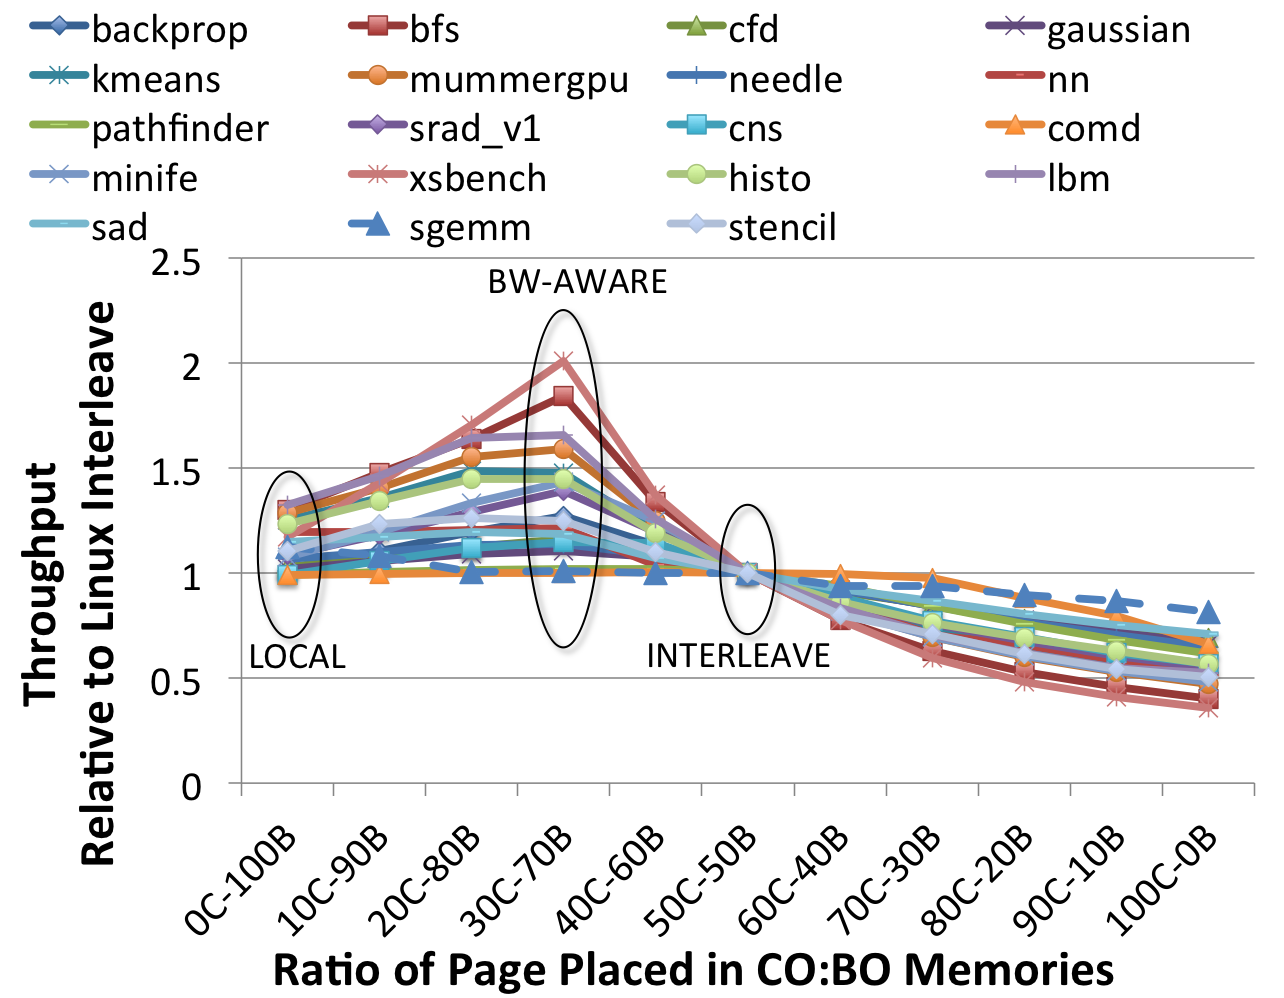
\includegraphics[width=0.9\columnwidth]{asplos2015/figures/bw-aware-2.png} 
    \caption{GPU workload performance with different page placement policies.
$xC$-$yB$ policy represents $x:y$ data transfer ratio from CO and BO memory respectively.}
    \label{fig:baseline}
\end{figure}

%\vspace{0.05in}
\subsection{BW-AWARE Performance: experimental results}
We define our BW-AWARE page placement policy $xC$-$yB$, where $x$ and $y$ denote the
percentage of pages placed in a given memory technology, $C$ stands for capacity-optimized
memory and $B$ stands for bandwidth-optimized memory. By definition $x+y=100$. For our baseline
system with 200GB/sec bandwidth-optimized memory and 80GB/sec of capacity-optimized memory the
aggregate system bandwidth is 280GB/sec.  In this
notation, our BW-AWARE policy will then be $x=80/280=28\%$ and $y=200/280=72\%$, represented as
$28C$-$72B$. However, for simplicity we will round this to $30C$-$70B$ for use as the 
placement policy.  For processes running on the GPU, the LOCAL policy
would be represented as $0C$-$100B$; $50C$-$50B$ corresponds to the bandwidth spreading Linux
INTERLEAVE policy.

To achieve the target $30C$-$70B$ bandwidth ratio, we implemented BW-AWARE placement as follows.
On any new physical page allocation, a random number in the range $[0,99]$
is generated.  If this number is $\geq30$, the page is allocated from the bandwidth-optimized memory; 
otherwise it is allocated in the capacity-optimized memory. A LOCAL allocation policy can avoid the
comparison if it detects either B or C has the value zero.  While this implementation does
not exactly follow the BW-AWARE placement ratio due to the use of random numbers, in practice this 
simple policy converges quickly towards the BW-AWARE ratio.  This approach also requires no history
of previous placements {\color{black} nor makes any assumptions about the frequency of access to pages}, 
minimizing the overhead for making placement decisions which are on the 
software fast-path for memory allocation.

Figure~\ref{fig:baseline} shows the application performance as we vary the ratio of pages placed in 
each type of memory from 100\% BO to 100\% CO\@. 
For all bandwidth-sensitive applications, the maximum performance is
achieved when using the correct BW-AWARE $30C$-$70B$ placement ratio.  We
find that, on average, a BW-AWARE policy performs 18\% better than the Linux
LOCAL policy and 35\% better than the Linux INTERLEAVE policy. However, for latency sensitive
applications, such as {\tt sgemm}, the BW-AWARE policy may perform worse than a LOCAL
placement policy due to an increased number of accesses to higher latency remote
CO memory. The BW-AWARE placement policy suffers a worse case performance degradation of
12\% over the LOCAL placement policy in this scenario.

%This degradation is expected
% since performance degrades by 9\% when the memory latency is 140 cycles
% (Figure~\ref{fig:latency}), which
% is very near to average memory latency (130 cycles = 70\%*100 + 30\%*200).}
%All of the applications we examined appear to be able to tolerate the additional 
%interconnect latency when using a remote capacity-optimized memory.

Because the current Linux INTERLEAVE policy is identical to BW-AWARE for a bandwidth-symmetric
DRAM $50C$-$50B$ memory technology pairing, we believe a BW-AWARE placement policy could simply
replace the current Linux INTERLEAVE policy without having significant negative side
affects on existing CPU or GPU workloads.  Because maximizing bandwidth is more important
than minimizing latency for GPU applications, BW-AWARE placement may be a good candidate
to become the default placement policy for GPU-based applications.
% It is worth noting that there are some GPU applications that are known to be
% sensitive to DRAM latency {\color{red}({\tt sgemm} in our case)}, 
% and using the LOCAL page placement policy may still be preferred.

\begin{figure}[t]
    \centering
    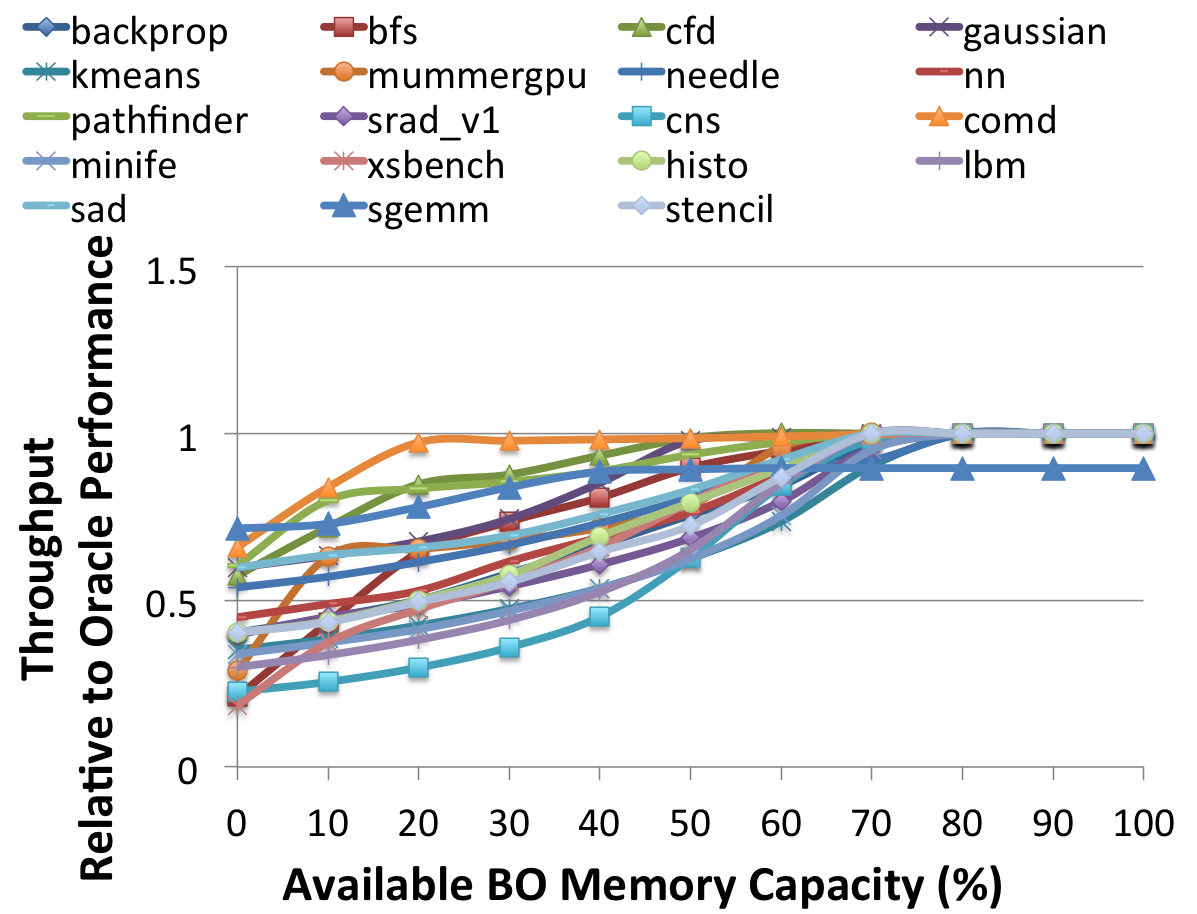
\includegraphics[width=0.9\columnwidth]{asplos2015/figures/bwaware-capacity.png}
    \caption{Performance of BW-AWARE placement as application footprint exceeds
available high-bandwidth
    memory capacity.}
    \label{fig:capacityconstrained}
\end{figure}

%\vspace{0.05in}
\subsubsection{Effective Improvement in Problem Sizing}
Figure~\ref{fig:capacityconstrained} shows the application throughput as we
reduce the capacity of our bandwidth-optimized memory pool as a fraction of the
total application footprint.  BW-AWARE placement is able to achieve near peak
performance even when only 70\% of the application footprint fits within the BO
memory because BW-AWARE placement places only 70\% of pages in BO memory, with
the other 30\% is placed in the less expensive capacity-optimized memory.  Thus,
GPU programmers who today tune their application footprint to fit entirely in
the GPU-attached BO memory could gain an extra 30\% effective memory capacity by
exploiting the CPU-attached CO memory with a BW-AWARE placement policy.
However, as the bandwidth-optimized memory capacity drops to less than 70\% of
application footprint, performance begins to fall off. This effect is due to the
ratio of bandwidth service from the two memory pools no longer matching the
optimal ratio of $30C$-$70B$, with more data being serviced from the capacity
optimized ratio than is ideal. Applications which are insensitive to memory
bandwidth (shown as having little change in Figure~\ref{fig:baseline}), tend to
maintain their performance at reduced capacity points (shown as having little
change in Figure~\ref{fig:capacityconstrained}), because the average bandwidth
reduction does not strongly affect their performance.  Conversely, those
applications with strong BW-performance scaling tend to see larger performance
reduction as the average bandwidth available is reduced, due to capacity
constraints forcing a disproportionate number of memory accesses to the lower
bandwidth CO memory.  The performance at 70\% memory capacity does not exactly
match 100\% of ideal because the actual ratio of bandwidth in our system is
$28C$-$72B$ not $30C$-$70B$.

\begin{figure}[t]
    \centering
    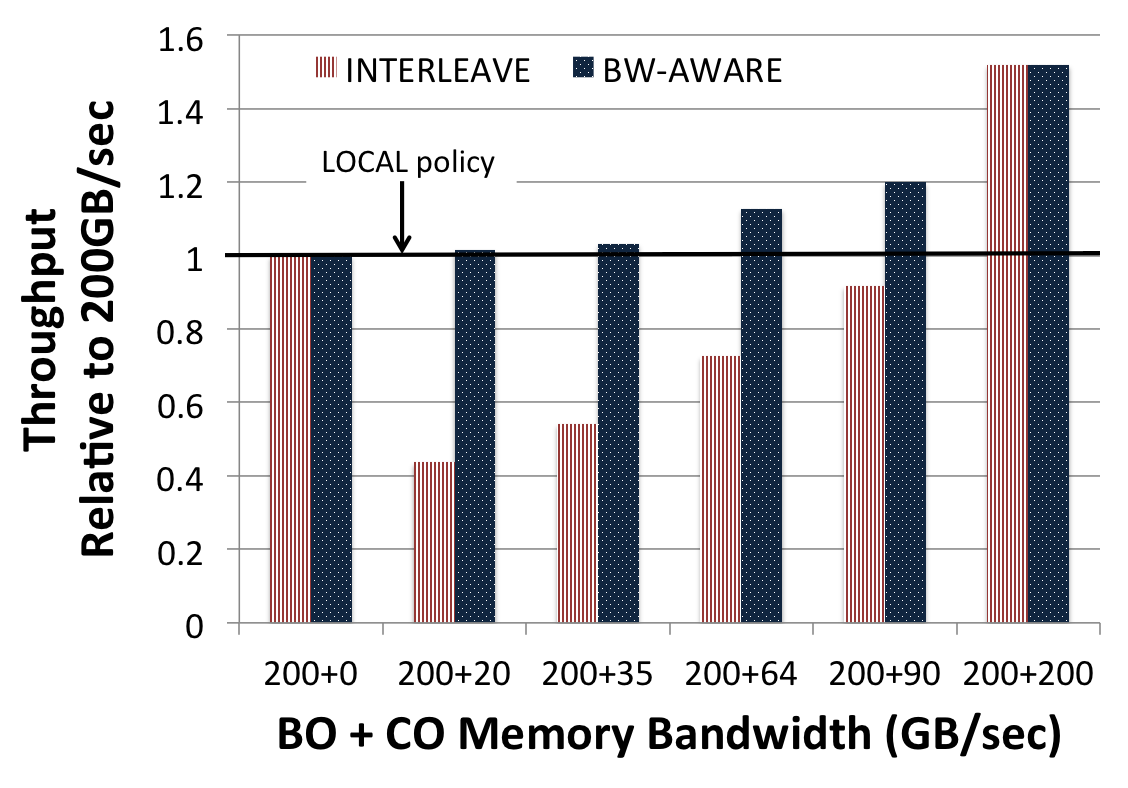
\includegraphics[width=0.9\columnwidth]{asplos2015/figures/sensitivitytobwratio.png}
    \caption{Performance comparison between BW-AWARE, INTERLEAVE, and LOCAL page placement
policies while varying the memory bandwidth ratio.}
    \label{fig:sensitivitytobwratio}
\end{figure}

%\vspace{0.05in}
\subsubsection{Sensitivity to NUMA BW-Ratios} 
Heterogeneous memory systems are likely to come in a variety of configurations.
For example, future mobile products may pair energy efficient and
bandwidth-optimized Wide-IO2 memory with cost-efficient and higher capacity
LPDDR4 memory.  Using the mobile bandwidths shown in
Figure~\ref{fig:arch-asplos2015}, this configuration provides an additional 31\%
in memory bandwidth to the GPU versus using the bandwidth-optimized memory
alone.  Similarly, HPC systems may contain GPUs with as many as 4 on-package
bandwidth-optimized HBM stacks and high speed serial interfaces to bulk capacity
cost/capacity-optimized DDR memory expanders providing just 8\% additional
memory bandwidth.  While we have explored BW-AWARE placement in a desktop-like
use case, BW-AWARE page placement can apply to all of these configurations.  

Figure~\ref{fig:sensitivitytobwratio} shows the average performance of BW-AWARE, INTERLEAVE, and LOCAL
placement policies as we vary the additional bandwidth available from the
capacity-optimized
memory from 0GB/s--200GB/s.
As the bandwidth available from capacity-optimized memory increases, the LOCAL policy
fails to take advantage of it by neglecting to allocate any pages in the capacity-optimized memory.
The Linux INTERLEAVE policy, due to its fixed round-robin allocation, loses performance
in many cases because it oversubscribes the capacity-optimized memory, resulting in less
total bandwidth available to the application.  On the other hand, BW-AWARE placement
is able to exploit the bandwidth from the capacity-optimized memory regardless the 
amount of additional bandwidth available.  Because BW-AWARE placement performs identically to
INTERLEAVE for symmetric memory and outperforms it in all heterogeneous cases, we believe that
BW-AWARE placement is a more robust default policy than INTERLEAVE when considering bandwidth-sensitive 
GPU workloads.
